% Copyright 2019 Robert Joslyn
% Unless otherwise noted:
%     Code (the LaTeX in this file) is licensed GPL-3.0 or later
%     Content (slide text and images) is licensed CC BY-SA 4.0

\documentclass[aspectratio=169]{beamer}
\usetheme{Rochester}

% Use Bera Mono font
\usepackage[T1]{fontenc}
\usepackage[scaled=0.8]{beramono}

% Remove navigation buttons
\setbeamertemplate{navigation symbols}{}

% Define SEL blue
\definecolor{SELblue}{HTML}{003b70}
\usecolortheme[named=SELblue]{structure}

\title{Building Custom Linux Systems with the Yocto Project}
\author[RJ]{Robert Joslyn}
\institute[SEL]{Schweitzer Engineering Laboratories}
\date[SeaGL]{Seattle GNU/Linux Conference, 2019}

\begin{document}

% Slide 1
\frame{\titlepage}

% Slide 2
\begin{frame}
\frametitle{Yocto Project}
\begin{itemize}
	\item It's not an embedded Linux distribution, it creates one for
	      you
	\item Automates downloading sources, cross-compiling, and
	      assembling images
	\item Uses tools and metadata co-developed with OpenEmbedded
	\item Includes a reference distribution called Poky
\end{itemize}
\end{frame}

% Slide 3
\begin{frame}
\frametitle{Yocto Project}
\begin{itemize}
	\item Robust framework for customization
	\item Auditing
	\begin{itemize}
		\item Build entire toolchain and final image from source
		\item Licensing
		\item CVE analysis
	\end{itemize}
	\item Easier hardware porting
	\item Community
\end{itemize}
\end{frame}

% Slide 4
\begin{frame}[fragile]
\frametitle{First Steps}
\begin{block}{}
\begin{semiverbatim}
$ git clone -b zeus git://git.yoctoproject.org/poky
$ cd poky
$ . oe-init-build-env
$ bitbake core-image-minimal
$ runqemu
\end{semiverbatim}
\end{block}
\end{frame}

% Slide 5
\begin{frame}
\frametitle{Shared State Cache}
Downloading and compiling an entire Linux system can take a long time.
Bitbake caches build artifacts to help ease the pain.
\begin{itemize}
	\item Source code is saved to a common directory: DL\_DIR
	\item Build artifacts are saved to sstate cache directory:
	      SSTATE\_DIR
	\item Can be shared between developers
	\begin{itemize}
		\item NFS
		\item HTTP/HTTPS
	\end{itemize}
\end{itemize}
\end{frame}

% Slide 6
\begin{frame}[fragile]
\frametitle{Customize}
Simple changes can be done in local.conf
\begin{block}{local.conf}
\begin{semiverbatim}
IMAGE\_INSTALL\_append = " vim"
\end{semiverbatim}
\end{block}
\begin{block}{Run the build}
\begin{semiverbatim}
$ bitbake core-image-minimal
$ runqemu
\end{semiverbatim}
\end{block}
\end{frame}

% Slide 7
\begin{frame}[fragile]
\frametitle{Customize More}
\begin{block}{local.conf}
\begin{semiverbatim}
IMAGE\_INSTALL\_append = " vim htop"
\end{semiverbatim}
\end{block}
\begin{block}{Run the build}
\begin{semiverbatim}
$ bitbake core-image-minimal
\end{semiverbatim}
\end{block}
\pause
\begin{block}{:-(}
\begin{semiverbatim}
ERROR: Nothing RPROVIDES 'htop' (but /home/robert/yocto/seagl2019/poky/
meta/recipes-core/images/core-image-minimal.bb RDEPENDS on or otherwise
requires it)
\end{semiverbatim}
\end{block}
\end{frame}

% Slide 8
\begin{frame}
\frametitle{Bitbake Layers}
\begin{itemize}
	\item Layers are software repositories
	\item Make reuse easier
	\item Allow placing recipes into logical groups
	\item A layer can modify recipes from another layer
\end{itemize}
\end{frame}

% Slide 9
\begin{frame}
\frametitle{OpenEmbedded Layer Index}
\begin{center}
	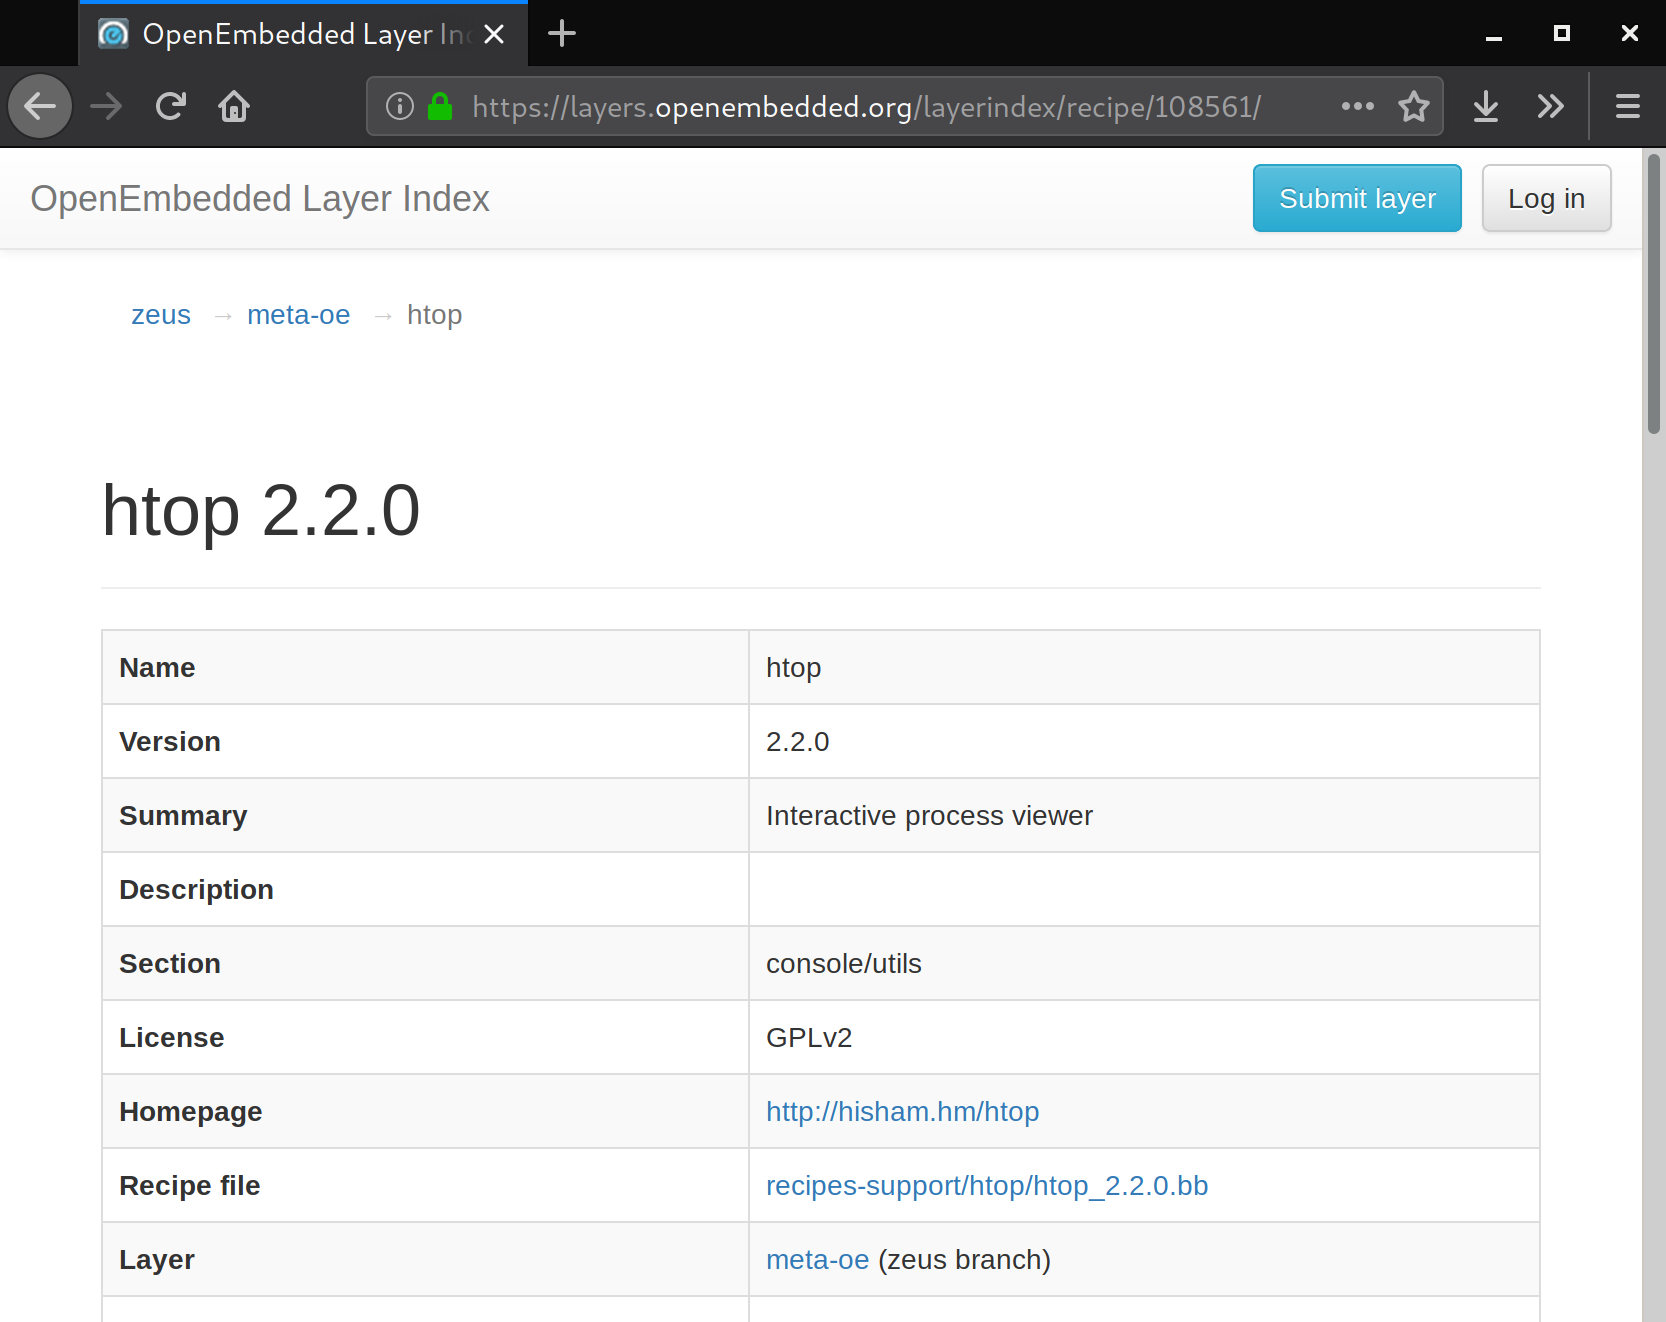
\includegraphics[width=\textwidth,height=0.9\textheight,keepaspectratio]{images/htop-layer-index.png}
\end{center}
\end{frame}

% Slide 10
\begin{frame}[fragile]
\frametitle{Use the Community}
\begin{block}{Clone another layer}
\begin{semiverbatim}
$ git clone -b zeus git://git.openembedded.org/meta-openembedded
\end{semiverbatim}
\end{block}
\begin{block}{bblayers.conf}
\begin{semiverbatim}
BBLAYERS += "/home/robert/yocto/seagl2019/poky/meta-openembedded/meta-oe"
\end{semiverbatim}
\end{block}
\begin{block}{Run the build}
\begin{semiverbatim}
$ bitbake core-image-minimal
$ runqemu
\end{semiverbatim}
\end{block}
\end{frame}

% Slide 11
\begin{frame}
\frametitle{How it Works}
\begin{itemize}
	\item bitbake parses layers for configuration and recipes, then
	      performs the build
	\item Layers contain recipes
	\item Recipes build packages
	\begin{itemize}
		\item Download and patch source code
		\item Set configure options
		\item Cross-compile
		\item rpm, ipk, or deb
	\end{itemize}
	\item Packages are assembled into images
\end{itemize}
\end{frame}

% Slide 12
\begin{frame}
\frametitle{Recipe Ingredients}
\begin{center}
	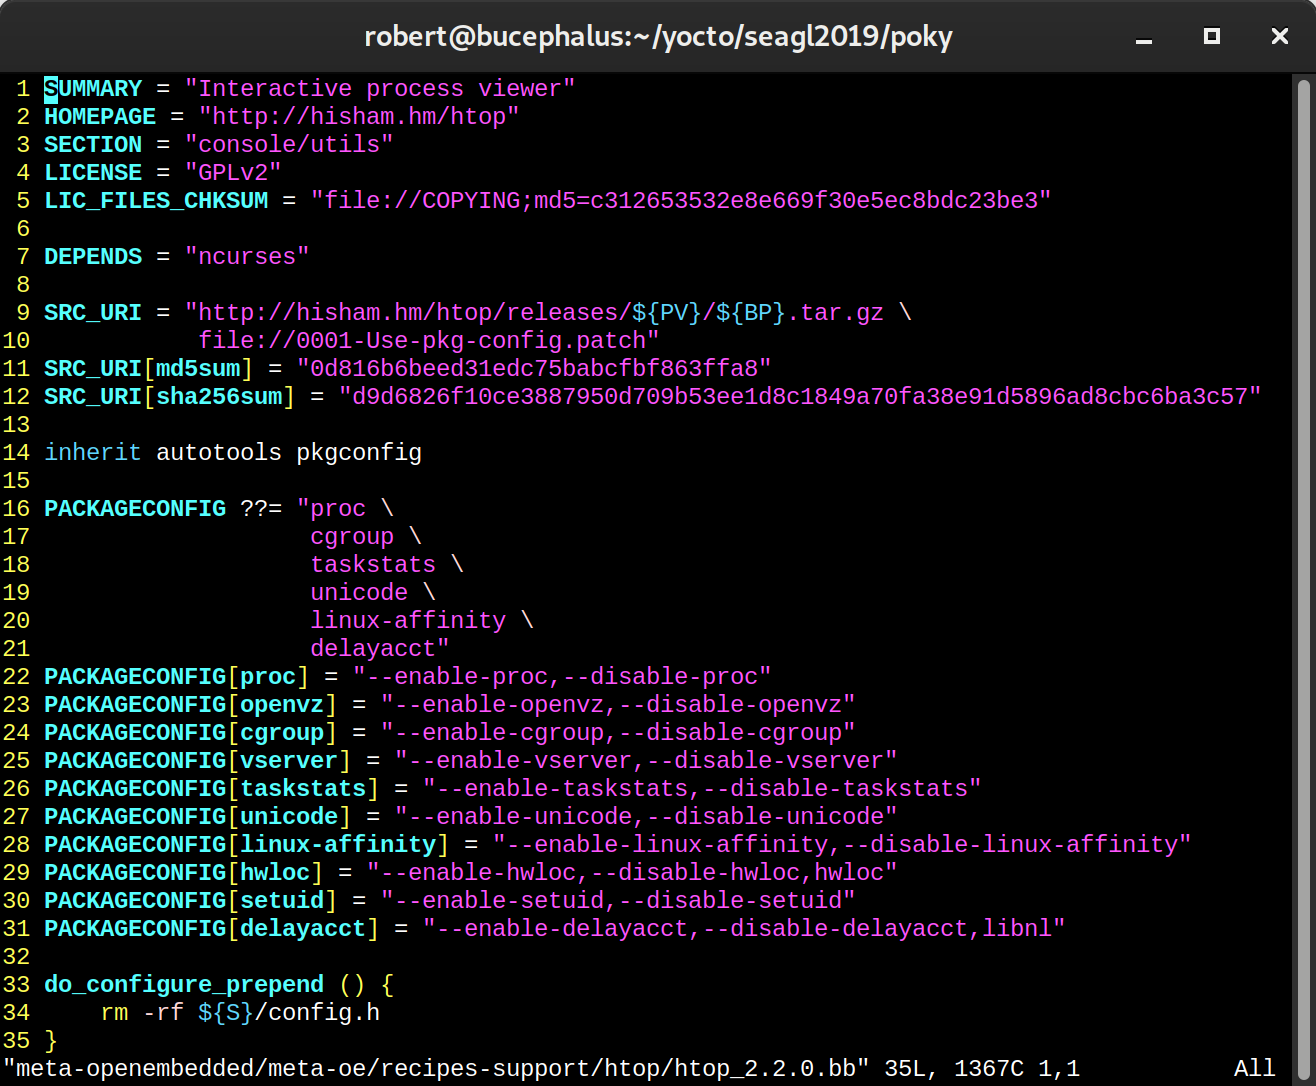
\includegraphics[width=\textwidth,height=0.9\textheight,keepaspectratio]{images/htop.png}
\end{center}
\end{frame}

% Slide 13
\begin{frame}[fragile]
\frametitle{Modify a Recipe from Another Layer}
Don't fork upstream layers. Modify recipes from your own layer.
\begin{block}{}
\begin{semiverbatim}
$ bitbake-layers create-layer ../meta-seagl
$ bitbake-layers add-layer ../meta-seagl
\end{semiverbatim}
\end{block}
Create a .bbappend file.
\begin{block}{}
\begin{semiverbatim}
mkdir -p ../meta-seagl/recipes-support/htop
vi ../meta-seagl/recipes-support/htop/htop\_\%.bbappend
\end{semiverbatim}
\end{block}
\end{frame}

% Slide 14
\begin{frame}[fragile]
\frametitle{Modify a Recipe from Another Layer}
\begin{block}{meta-seagl/recipes-support/htop/htop\_\%.bbappend}
\begin{semiverbatim}
PACKAGECONFIG = "proc"
\end{semiverbatim}
\end{block}
\begin{block}{meta-seagl/recipes-support/htop/htop\_\%.bbappend}
\begin{semiverbatim}
PACKAGECONFIG\_append = " hwloc"
\end{semiverbatim}
\end{block}
\begin{block}{meta-seagl/recipes-support/htop/htop\_\%.bbappend}
\begin{semiverbatim}
PACKAGECONFIG\_remove = "delayacct"
\end{semiverbatim}
\end{block}
\end{frame}

% Slide 15
\begin{frame}
\frametitle{Recipe WORKDIR}
\begin{center}
	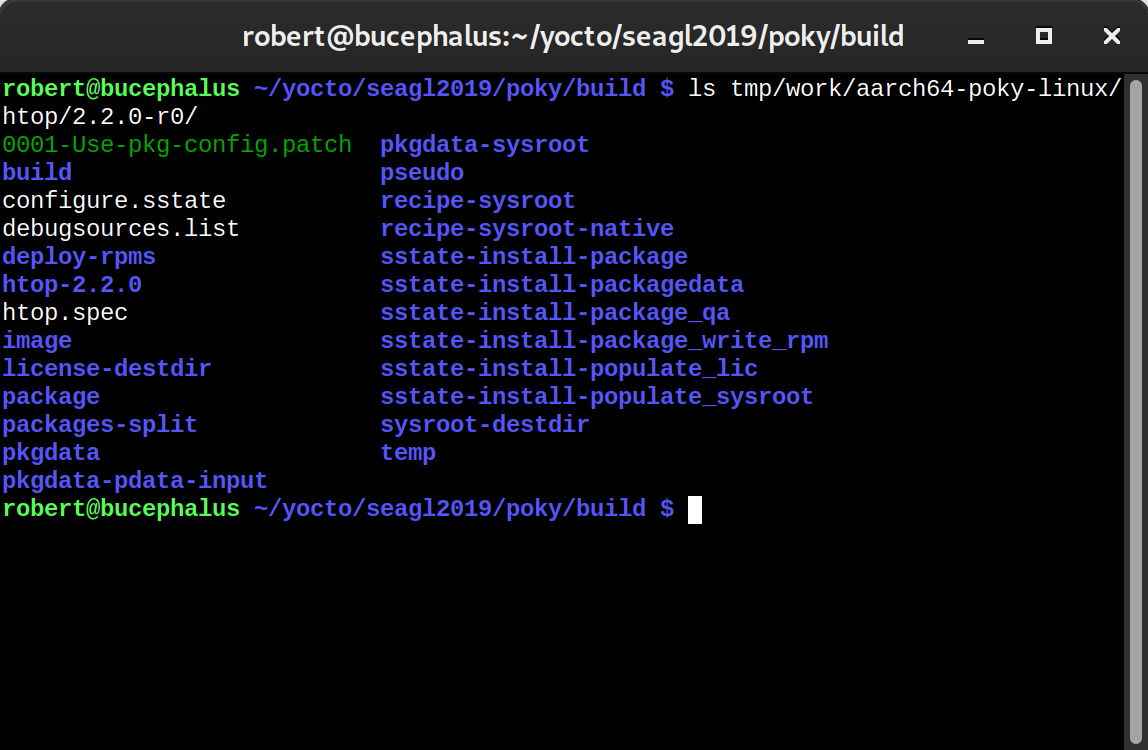
\includegraphics[width=\textwidth,height=0.9\textheight,keepaspectratio]{images/htop-workdir.png}
\end{center}
\end{frame}

% Slide 16
\begin{frame}
\frametitle{Package Content}
\begin{center}
	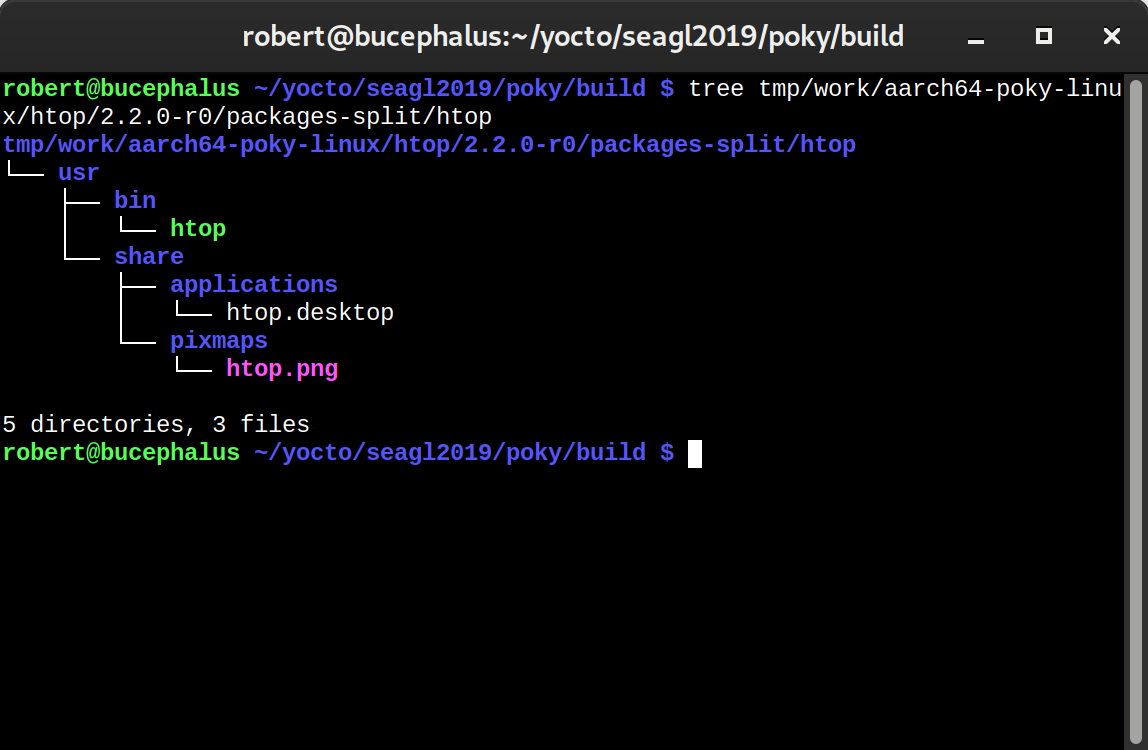
\includegraphics[width=\textwidth,height=0.9\textheight,keepaspectratio]{images/htop-packages-split-before.png}
\end{center}
\end{frame}

% Slide 17
\begin{frame}[fragile]
\frametitle{Modify Package Content}
Remove files from package
\begin{block}{meta-seagl/recipes-support/htop/htop\_\%.bbappend}
\begin{semiverbatim}
do\_install\_append() \{
    rm -r $\{D\}$\{datadir\}
\}
\end{semiverbatim}
\end{block}
\end{frame}

% Slide 18
\begin{frame}
\frametitle{Modify Package Content}
\begin{center}
	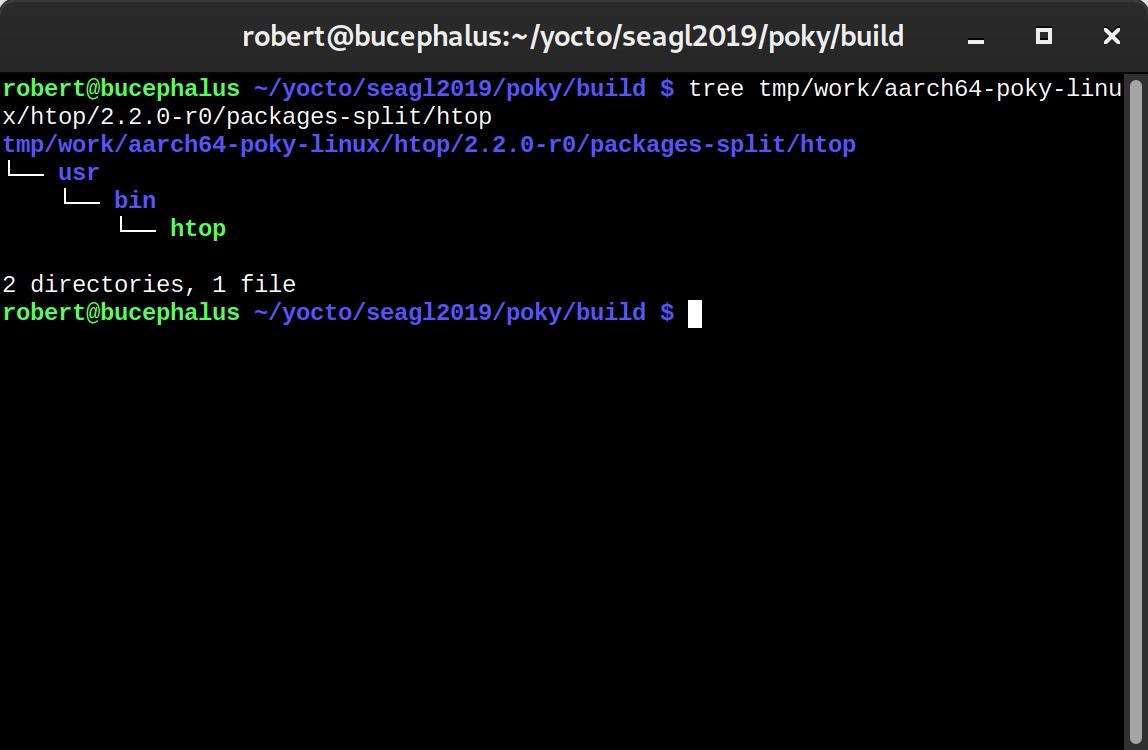
\includegraphics[width=\textwidth,height=0.9\textheight,keepaspectratio]{images/htop-packages-split-after.png}
\end{center}
\end{frame}

% Slide 19
\begin{frame}
\frametitle{Larger Changes}
\begin{itemize}
	\item MACHINE
	\begin{itemize}
		\item Select hardware platform
		\item Impacts compile options, kernel options, and potentially anything that is hardware specific
	\end{itemize}
	\item DISTRO
	\begin{itemize}
		\item Sets distro-wide policy
		\item Should applications build GUIs?
		\item sysvinit or systemd?
		\item Recipes can inspect DISTRO\_FEATURES to enable or
		      disable features
	\end{itemize}
	\item IMAGE\_FEATURES
	\begin{itemize}
		\item Should debug, source, or dev packages be installed?
		\item Debug or release build?
	\end{itemize}
\end{itemize}
\end{frame}

% Slide 20
\begin{frame}[fragile]
\frametitle{Booting Real Hardware}
\begin{block}{local.conf}
\begin{semiverbatim}
MACHINE = "genericx86-64"
IMAGE\_FSTYPES\_append = " wic"
WKS_FILE = "mkefidisk.wks"
\end{semiverbatim}
\end{block}
More wks examples are in \texttt{poky/scripts/lib/wic/canned-wks/}
\begin{block}{Write to disk}
\begin{semiverbatim}
$ dd if=tmp/deploy/images/genericx86-64/core-image-minimal.wic \\
     of=/dev/sdb bs=1M
\end{semiverbatim}
\end{block}
\end{frame}

% Slide 21
\begin{frame}[fragile]
\frametitle{Changing init}
Generally the DISTRO selects the init manager. Poky defaults to sysvinit,
but this can be overridden.
\begin{block}{local.conf}
\begin{semiverbatim}
DISTRO\_FEATURES\_append = " systemd"
VIRTUAL-RUNTIME\_init\_manager = "systemd"
# Remove initscripts entirely from the image
DISTRO\_FEATURES\_BACKFILL\_CONSIDERED = "sysvinit"
VIRTUAL-RUNTIME\_initscripts = ""
\end{semiverbatim}
\end{block}
\end{frame}

% Slide 22
\begin{frame}[fragile]
\frametitle{Tracking Changes}
The buildhistory class captures metadata for build and can commit to a git
repository. This helps see how changes impact the image as a whole.
\begin{itemize}
	\item Files in images and packages
	\item File sizes and permissions
	\item Package dependencies
\end{itemize}
\begin{block}{local.conf}
\begin{semiverbatim}
INHERIT += "buildhistory"
BUILDHISTORY\_COMMIT = "1"
\end{semiverbatim}
\end{block}
\end{frame}

% Slide 23
\begin{frame}
\frametitle{Resources}
Yocto has extensive documentation
\begin{itemize}
	\item \url{https://yoctoproject.org}
	\item \url{https://yoctoproject.org/docs/latest/mega-manual/mega-manual.html}
	\item \url{https://yoctoproject.org/community/mailing-lists/}
	\item \url{https://layers.openembedded.org/layerindex/branch/zeus/recipes/}
\end{itemize}
\LaTeX{} source code for this presentation is available on my website:
\begin{itemize}
	\item \url{https://git.robertjoslyn.com/seagl2019/}
	\item \url{robert.joslyn@redrectangle.org}
\end{itemize}
\end{frame}

\end{document}
